

\documentclass[10pt]{article}

\usepackage{amssymb}
\usepackage{amsmath}
\usepackage{amsthm}
\usepackage[pdftex]{graphicx}
\usepackage{multirow}
\usepackage{float}
\newtheorem{thm}{Theorem}



\begin{document}

\begin{center}

{\bf Computing the Log Concave NPMLE for Interval Censored Data}


	Clifford Anderson-Bergman
	
	Yaming Yu
	
\end{center}

{\section {Abstract}}

	In analyzing interval censored data, a non-parametric estimator is often desired, due to difficulties in assessing model fits. Much work has been put into the computation of the non-parametric estimator. However, the estimates for values of interest of the survival function, such as the quantiles, have very large standard errors due to the jagged form of the estimator. By forcing the estimator to be constrained to the class of log concave functions, we insure a once differentiable survival estimator which has much better operating characteristics than the unconstrained NPMLE. In this paper, we focus on an algorithm for computing the log concave NPMLE. Using simulated data, we see that this new estimator has very favorable operating characteristics compared to the unconstrained NPMLE and another competing estimator for interval censored data. We will apply the algorithm to current status data for the onset of menopause. 

{\section{Introduction}}

	Interval censored data can occur when the time to event is known only up to an interval, \emph{i.e.} the $i^{th}$ event time is only known to have occurred after $L_{i}$ and before $R_i$. A special case of interval censoring that will be examined is case I interval censored data, or current status data. In this case, each subject $i$ is observed at a random time $C_i$. The only information collected is whether the event of interest has occurred before $C_i$ (in which case $L_i$ = 0 and $R_i$ = $C_i$) or the event has not occurred by time $C_i$ (in which case $L_i$ = $C_i$ and $R_i$ = $\infty$).
	
	For such data, model assessment can be very difficult, as visual plots such as histograms cannot be used. As a result, there is high demand for non parametric estimators, which tend to rely less heavily on assumptions of the data. The non-parametric maximum likelihood estimator (NPMLE) has been studied in depth (Turnbull 1976, Gentleman and Geyer 1994, Huan and Wellner 1997, Jongbloed 1998) and is often the estimator of choice. This will be referred to as the unconstrained NPMLE for the remainder of this article. The unconstrained NPMLE has been shown to be consistent for the survival distribution in the univariate case (Gentleman and Geyer 1994). However, for any finite sample size, the estimator shows erratic jumps (see figure 1), making any density estimate degenerate and resulting in a slow convergence of the estimated survival distribution, at the rate of $n^{-1/3}$ instead of the more typical $n^{-1/2}$ (Huan and Wellner 1997). 
	
\begin{figure}[h]
\centerline{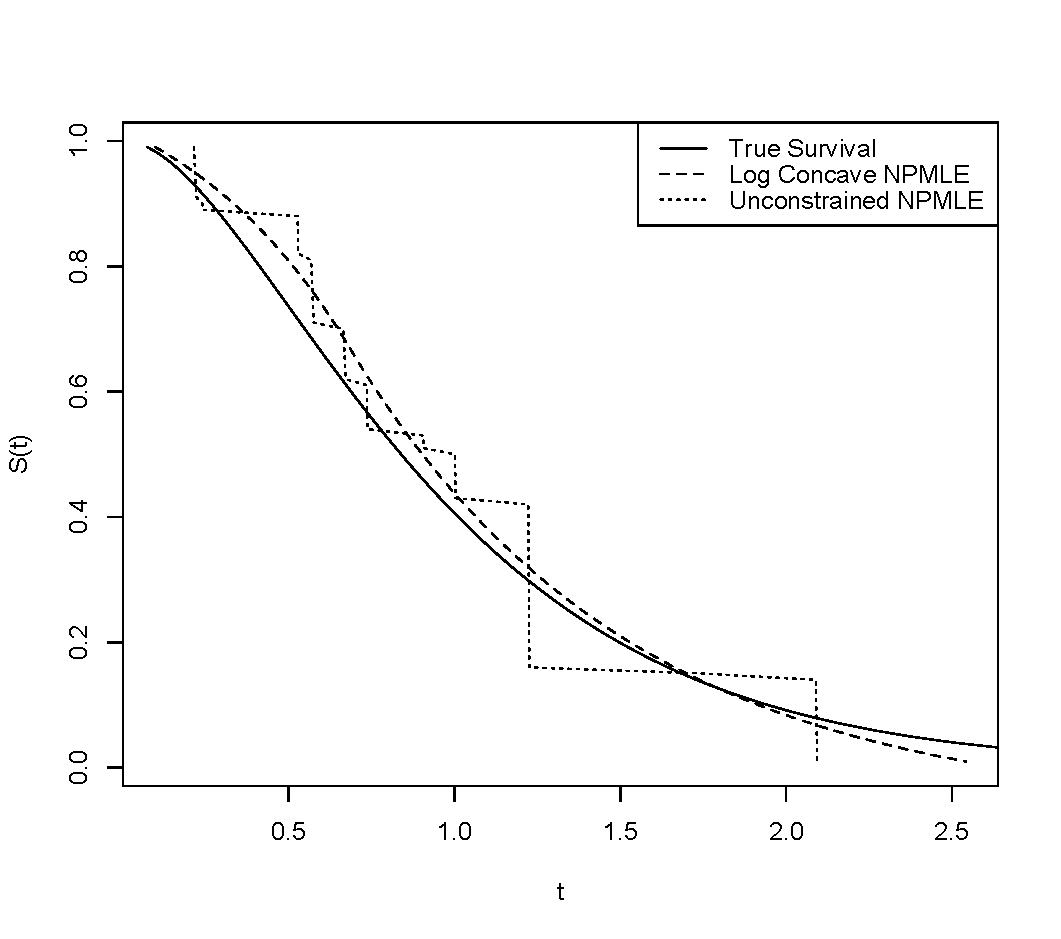
\includegraphics[width = 7cm]{LCvUC.pdf} }
\caption{Log concave NPMLE and unconstrained NPMLE. Data is current status data simulated from a Gamma(2,2) distribution with $n = 400$ }
\end{figure}		
			
	Attempts have been made to achieve a smoother estimator in order to improve operating characteristics. One technique is smoothing over the unconstrained NPMLE with a kernel estimator (Betensky et al 1999). Another technique is to model the density with log-spline functions, using AIC to select the number of knots (Kooperberg and Stone, 1992). While both of these techniques have been shown to reduce the variance of the estimated survival curve for interval censored data (Wei Pan 2000), they have their drawbacks as well. Both these estimators require selecting some sort of smoothing parameter, which can be non-trivial in the interval censored case. As an example, the log spline density estimator can be found in the CRAN package  ``logspline", with preset smoothing penalties. While this estimator can preform well with light censoring, in our experience with simulated data, the estimator behaves very poorly under heavy censoring. In particular, it was often observed either the estimate of the density jumps highly erratically or the algorithm fails to converge when used with current status data, even for large data sets (in fact, the estimator appears to preform \emph{worse} for large data sets). Similar problems were noted in Wei Pan 2000.  Likewise, the question of bandwidth selection for the kernel smoother for interval censored data is still an open question. While there are ad-hoc selection methods available, more work is still needed and this does produce demand for a fully automated, theoretically justified smooth estimator.
	
	In most studies, the survival function is believed to be smooth. Many researchers have investigated using various smoothness assumptions (rather than smoothness parameters) to improve the operating characteristics of the estimator. An early example of such an estimate is that of a non-increasing density (Grenander 1956). An extension of the non-increasing density is the uni-modal density (non-decreasing before the mode, non-increasing after), but the uni-modal NPMLE has been shown to be inconsistent at the mode (Wegman 1969). Another popular shape constraint is that of log concavity (Bagnoli and Bergstorm 2005). This assumption is considered very flexible as many parametric distributions fit into this category. The families of log concave distributions include normal, gamma with shape parameter $\ge$ 1, all Weibull densities with exponent $\ge$1, all beta densities with both parameters $\ge 1$ and the logistic density. Non-logconcave distributions include the t-distribution, the lognormal distribution and any multimodal distribution. However, the log concave estimator has been shown to be very useful in mixture modeling (Chang and Walther 2007) so it can be useful for multimodal data as well. This estimator has been shown to be a consistent estimator of density in the case of exact data (D\"umbgen and Rufibach 2009) and an efficient algorithm for finding the log concave NPMLE has been written for exact data (Rufibach 2007). 
	
	
	The problem is much more difficult for interval censored data. At the same time, there is more utility in a log concave estimator for interval censored data than in the case of exact data. By forcing the estimated density to be log concave, a fairly flexible assumption, one can greatly improve the operating characteristics of the estimated survival function without having to make more limiting assumptions of families of parametric distributions which can be very difficult to assess for interval censored data. However, computing the NPMLE is challenging for this case. Currently, there is an EM algorithm which requires discretizing the data and thus estimates an approximation (D\"umbgen et al 2011). In this paper, we are interested in using the exact times. In order to solve for an exact solution, a theorem for restricting the solution to a finite number of parameters is required. Once a finite support set is obtained, likelihood functions involving interval censored data often are not strictly concave, making maximization very difficult (the reader must be very careful to note the distinction between the log likelihood being concave and the estimator being log concave). In this paper, we prove a theorem for reducing the number of parameters required to characterize the log concave NPMLE to a finite set and an algorithm for finding a log concave NPMLE solution over those parameters. It is worth noting that the algorithm presented in this paper is considerably faster than the discrete approximation in its current form. For $n = 25$, the discrete approximation took on average 12 seconds, while the algorithm we present took on average 0.21 seconds. For $n = 50$, the discrete approximation took 31 seconds, while ours took 0.44 (simulations were done in R, using a Macbook with a 2GHz Intel Core 2 Duo processor with 4 GB of RAM. Our algorithm was written in R and theirs was provided in the CRAN package ``logconcens"). Solutions were visually identical. It is worth noting that D\"umbgen et al state that their algorithm may be very slow due to an over sensitive stopping criterion. Average times for our algorithm for larger data sets will be presented later.
	
	In section 3, we introduce the likelihood function that we are interested in maximizing. In section 4, we prove a theorem which shows that the maximum likelihood can be achieved by a function of a finite number of parameters. In section 5, we describe the convergence criterion for this problem. In section 6, we outline the algorithm. In section 7, we apply the algorithm to a classic sample data set and compare the results to that of the unconstrained NPMLE and the kernel smoother. In section 8, we simulate data and compare the bias and standard deviations of the log concave NPMLE, the unconstrained NPMLE and the kernel smoother across several different simulation scenarios. In section 9, we discuss future research topics for the log concave NPMLE.
	 
{\section {Likelihood}}

	For the $i^{th}$ subject, the exact event time is known to be within the observed interval $[L_i, R_i]$. Let $\phi(x)$ represent the log density at time $x$.  Assuming independence of observations and an independent censoring mechanism, the log concave NPMLE is 
	
	\[ \hat \phi(x) =\underset{\phi(x)} {\arg \max} \displaystyle \sum_{i = 1}^n \log \left( \int_{L_i}^{R_i} e^ { \phi(x) } \,dx \right)
	\]
	\[
	 s.t. \frac{ \phi(x_2) - \phi(x_1)} {x_2 - x_1} \geq \frac{ \phi(x_3) - \phi(x_2)} {x_3 - x_2} \hspace{0.5cm} \forall x_1 < x_2 < x_3 
	 \]
	 \[ \int_{-\infty}^{\infty} e^{\phi (x) } \,dx = 1
		\]

	In order to ease the last restriction, $e^{\phi(x)}$ is replaced with $\frac{e^{\phi(x)} } { \int  e^{\phi(x)} dx}$, so that $e^{\hat \phi(x)}$ is proportional to the LC NPMLE. Under this reparameterization, the LC NPMLE is written as 

	\[ \hat \phi(x) = \underset{\phi(x)} {\arg \max} \displaystyle \sum_{i = 1}^n \log \left( \int_{L_i}^{R_i} e^ { \phi(x) } \,dx \right) - n \times \log \left(  \int_{-\infty}^{\infty} e^ { \phi(x) } \,dx \right) 
	\]
	\[
	 s.t. \frac{ \phi(x_2) - \phi(x_1)} {x_2 - x_1} \geq \frac{ \phi(x_3) - \phi(x_2)} {x_3 - x_2}\hspace{0.5cm} \forall x_1 < x_2 < x_3 
	 \]
	
	It is worth noting that under this parameterization, $\hat \phi(x)$ is calculated up to an additive constant. While this is not a problem in computation, for simplicity we will set $\underset{x} {\arg \max}$ $\phi(x) = 0$. With this parameterization, we can interpret $\phi(x)$ as the log ratio between the density at $x$ and the density at the mode.

	It is worth noting that the restrictions do not insure that $\phi(x)$ is differentiable, but it does insure that $\phi(x)$ is continuous on the closed interval for which $e^{\phi(x)} > 0$. This implies that the estimated survival function will be once differentiable on $\mathbb{R}$, although not necessarily twice differentiable.
	
	In contrast, the unconstrained NPMLE is defined as 

	\[ \hat \phi(x) =\underset{\phi(x)} {\arg \max} \displaystyle \sum_{i = 1}^n \log \left( \int_{L_i}^{R_i} e^ { \phi(x) } \,dx \right)
	\]
	 \[ \int_{-\infty}^{\infty} e^{\phi (x) } \,dx = 1
		\]
	
	It has been shown that the solution to the unconstrained NPMLE assigns a certain mass to certain intervals called Turnbull intervals (Turnbull 1976) or maximal intersections. How mass is assigned within a Turnbull interval does not affect the likelihood value, so it is treated as a discrete problem, i.e. the problem can be reparameterized and maximized over the set $p$ such that $p_i = \int_{t_i}^{t_{i+1}} e^ { \phi(x) } \,dx$  for a certain set $t$. However, in the log concave NPMLE, the log concave restriction implies that how mass is assigned within a maximal intersection affects how the function will behave outside of the interval, so this problem does not have the same luxury of being able to optimize over such a reparameterization.
		
{\section{Solution Set}}

	In the case of exact observations, it has been shown that the log concave NPMLE must be a log piecewise linear function, with knots at the observed times and density of 0 outside the minimum and maximum observed times. (Rufibach 2007). To prove this, consider that for exact times the log likelihood function can be written as
	
	\[ \displaystyle \sum_{i = 1}^n \phi(x_i) - n \times \log \int e^{\phi(x)} dx
	\]
	
	For any set of values of $\phi(x_i)$, the likelihood is maximized by minimizing $\int e^{\phi(x)}$. If $x_i$ are the order statistics, then we note that for a fixed $\phi(x_i)$ and $\phi(x_{i+1})$, $\int_{x_i}^{x_{i+1}} e^{\phi(x)}dx$ under the concave restriction of $\phi(x)$ is minimized by linearly connecting $\phi(x_i)$ and $\phi(x_{i+1})$. Thus, $\hat \phi(x)$ is a log linear piecewise function in the case of exact observations. The concavity of the likelihood function with exact observations insures that the solution will be unqiue.
		
	In the case of interval censored data, the LC NPMLE is not necessarily unique. As a trivial example, consider the case n = 1. In such a case, any log concave function which places all of the mass inside of the observed interval would be an LC NPMLE. This is very similar to the problem of representational non-uniqueness in the unconstrained case (Gentleman and Vandal 2002). Issues with non-uniqueness will be briefly discussed in section 9. With such issues in mind, we will instead show that the maximum likelihood can be obtained via a log piecewise linear function with a finite number of knots, while recognizing that there may be other functions which achieve the same likelihood. 

\hspace{2mm}

	%{\subsection{Theorem}}
	\begin{thm}
	The maximum likelihood for the logconcave NPMLE can be achieved with a piecewise linear function with at most $4n-1$ knots.
	\end{thm}
\hspace{2mm}	
	
\begin{figure}[h]
\centerline{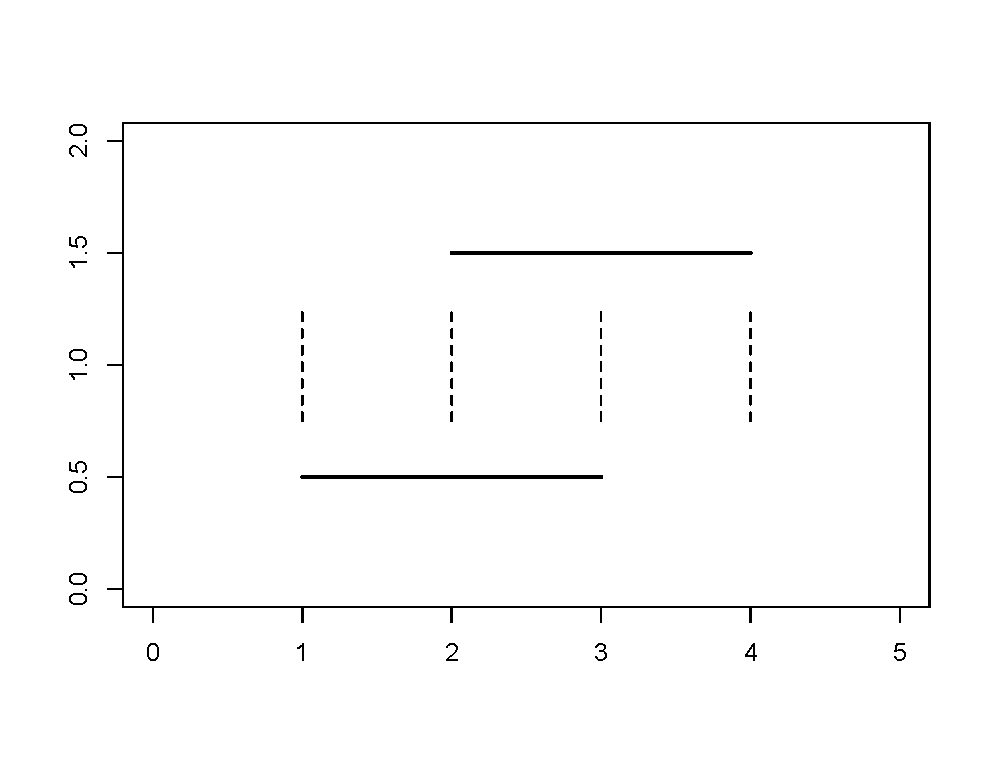
\includegraphics[width = 6cm]{ContrbInt.pdf} }
\caption{Observation intervals and contribution intervals}
\end{figure}	

	\begin{proof}

	Define the $i^{th}$ observation interval to be the interval in which the $i^{th}$ time was known to have occurred, i.e. the $i^{th}$ observation interval would be $[L_i, R_i]$. Define a contribution interval to be an interval such that both ends of the interval are ends of an observation interval, with no other ends of observation intervals in between. For example, figure 2 shows two observation intervals, $L_1 = 1$, $R_1 = 3$ and $L_2 = 2$, $R_2 = 4$. This leads to 3 contribution intervals; [1,2], [2,3] and [3,4]. Note that exchanging mass \emph{between} contribution intervals will affect the likelihood function, but exchanging mass \emph{within} will not. It should be noted that in all area that is not in a contribution interval, $\phi(x)$ needs to be minimized in the LC NPMLE. Thus, $\hat \phi(x)$ will be linear in areas that are between contribution intervals but are not contribution intervals and $\hat \phi(x)$ will be $-\infty$ in areas that are not contribution intervals and not between contribution intervals. 

	For the $k^{th}$ contribution interval, define $l_k$ and $r_k$ to be the end points. Note that for a given $\phi(l_k)$, $\phi'(l_k -)$ (left derivative at $l_k$), $\phi(r_k)$ and $\phi'(r_k+)$ (right derivative at $r_k$), the only way the contribution interval affects the likelihood is the total mass assigned to contribution interval $k$, $i.e.$ $p_k = \int_{l_k}^{r_k} e^ {\phi(x)} dx$ (note: under this parameterization, it is not necessary that $\sum p_k = 1$). It should be noted that $p_k$ is minimized by making $\phi(x)$ linear on $(l_k, r_k)$. If $\phi'(l_k - )$ = $\phi'(r_k + )$, then by concavity $\phi(x)$ must be linear over $(l_k, r_k)$ and no support points will be needed in the interval. If not, we will need to add another support point. Let us define a point inside the contribution interval 

	
	\[ m_k = \frac{\phi(r_k) - \phi'(r_k + ) r_k - \phi(l_k) + \phi'(l_k - ) l_k} { \phi'(l_k - ) - \phi'(r_k + )}
	\]

\begin{figure}[h]
\centerline{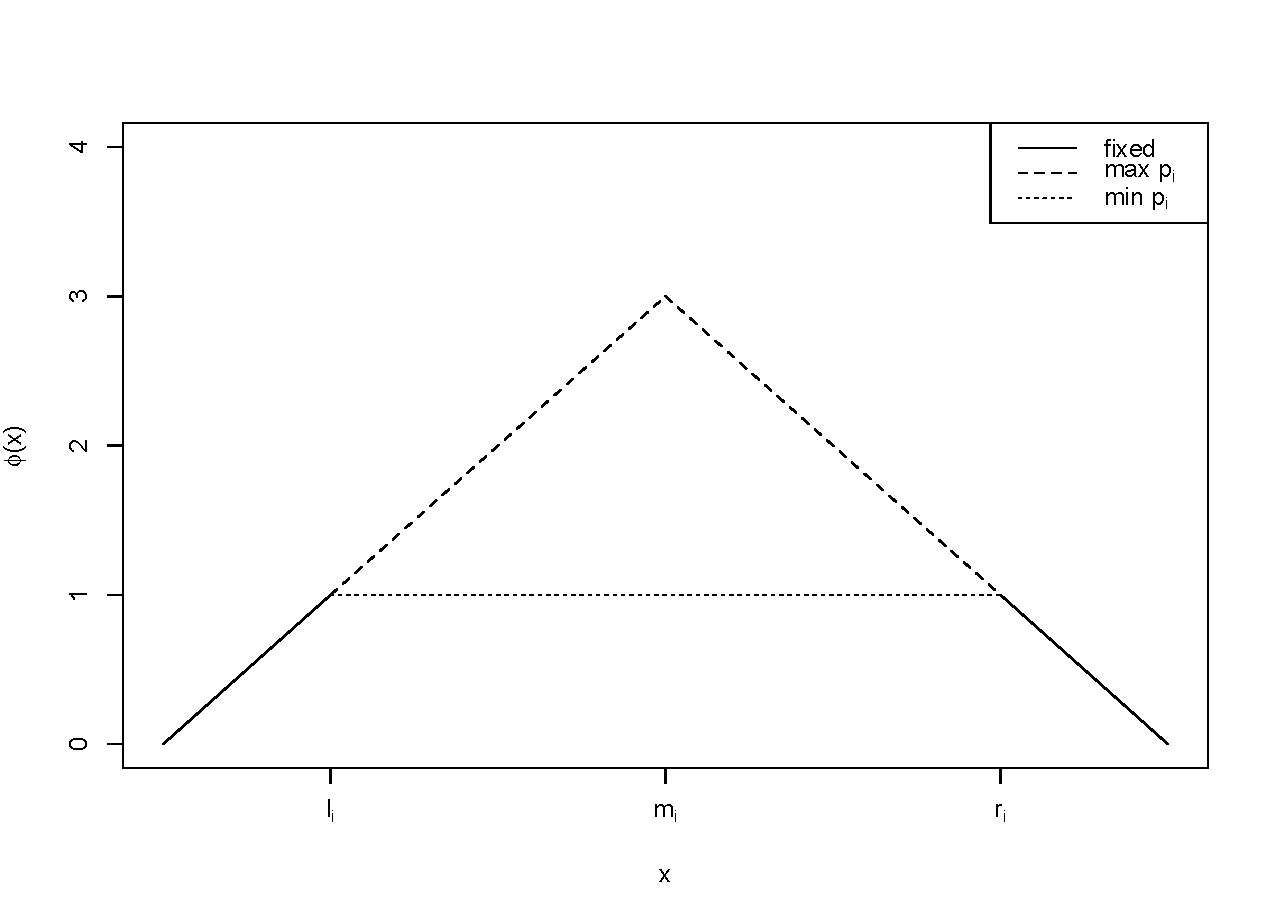
\includegraphics[width = 6cm]{maxminpk.pdf}}
\caption{Maximizing and Minimizing $p_k$}
\end{figure}		
	
	
	In other words, $m_k$ is the intersection of the linear expansions of $\phi(x)$ from $l_k$ and $r_k$. We can maximize $p_k$ by setting $\phi(m_k)$ to the value of this intersection, as seen in Figure 3. Therefore, by adding a knot at $m_k$, we can set $p_k$ to either the minimum or the maximum possible under the constraint of log concavity and a given $\phi(l_k)$, $\phi'(l_k -)$, $\phi(r_k)$ and $\phi'(r_k+)$. Also, we can set $p_k$ to any value between the minimum and maximum by setting $\phi(m_k)$ to any value between the minimum and maximum allowed by the constraints . Thus, if $\Phi$ is the set of piecewise linear functions with knots at the end points contribution interval and one knot inside each contribution interval, $\hat\phi(x) \in \Phi$. 
	
	\end{proof}
	
	A nuisance to be noted about this theorem is that without knowing $\hat\phi(x)$, one cannot know the exact location of $m_k$ for the $k^{th}$ contribution interval. This could be dealt with by finding the location of knots within intervals that maximize the likelihood function. However, this is likely to be very computationally expensive for very small difference in the estimated values. Instead, $m_k$ will be replaced with $mid_k = \frac{l_k + r_k}{2}$, which is likely to be very close $m_k$ and so an approximation of the log concave estimator will be found. Because this set of knots provides a very fine grid of knots without removing any information provided from each observation interval, it is unlikely that this approximation will be significantly different that the exact log concave NPMLE. For the rest of the paper, the support set will refer to all end points and mid points of all the contribution intervals.

	
	{\section{Stopping Criterion} } 
	
	A necessary (although not sufficient) condition for an estimate to be a global max is that it must satisfy the KKT conditions (Kuhn, Tucker 1951). A naive set of conditions to consider would be based on $\frac {dl}{d\phi(x_s)}$, where $x_s$ are from the support set in the above given theorem. Although satisfying these would be necessary for a global max, it would be a poor choice of stopping criterion for two reasons. Consider that for any region where $\phi(x)$ is a straight line, all points within the line are constrained from increasing or decreasing by the concavity constraint, even though the current estimate of the density at that region may be very far away from the density in the log concave NPMLE. So despite the current estimate of the density being far from that in the maximum, that particular point would be on the boundary (i.e. could not increase or decrease without increasing or decreasing neighboring density estimates) and so would have reported KKT error of 0. Secondly, because the $x_s$ form a fine grid, the change of an individual $\phi(x_s)$ in unlikely to have a large effect on the likelihood function. Thus, a stopping criterion based on the KKT conditions of this parameterization will not accurately portray how far the current estimate is from the max and will likely stop prematurely for any reasonable tolerance level $\epsilon$. 
	
	Instead, we will consider a ``pivot" transformation of $\phi(x)$. By pivorting $\phi(x)$ about $x_0$, we mean a change in the slope of $\phi(x)$ at $x_0$. If $x_i$ was selected and it was decided to pivot by $\delta_i$, then
	
	\[ \phi^{k+1}(x) = \phi^{k}(x); x \leq x_i
	\]
	
	\[ \phi^{k+1}(x) = \phi^{k}(x) + \delta_i \times (x - x_i) ; x > x_i
	\]

	Examining the KKT conditions is much more practical in this parameterization. We note that at each $x_i$, $\delta_i$ is only bounded from above, but not below. That is, $\delta_i$ can only be has high as the change in derivative at $x_i$, but can go as low as possible. In addition, changing $\phi(x)$ is in this manner will have a significant effect on the likelihood function. 
	
	We also use a backwards pivot, where $\phi(x)$ to left is pivoted and $\phi(x)$ to the right is fixed. In other words, if $x_i$ was selected and pivoted by $\delta_i$, then 

	\[ \phi^{k+1}(x) = \phi^{k}(x); x \geq x_i
	\]
	
	\[ \phi^{k+1}(x) = \phi^{k}(x) + \delta_i \times (x - x_i) ; x < x_i
	\]



	Based on this, we define the KKT error at $x_i$ as the absolute value of $\frac {dl} {d\delta_i}$ if $\phi(x_i)$ is on not on the boundary (i.e. $\phi_{(-)}'(x_i) > \phi_{(+)}'(x_i)$) and the maximum of $\{0, -\frac {dl} {d\delta_i} \}$ if $\phi(x_i)$ is on the boundary ($\phi_{(-)}'(x_i) = \phi_{(+)}'(x_i)$).Numerical problems make it challenging to determine whether a point in on the boundary. Instead, a point is considered to be on the boundary if $| \phi_{(-)}'(x_i) - \phi_{(+)}'(x_i) | < 10^{-10}$. Our stopping criterion, $err$, will be the maximum KKT error (considering both forward and backward pivots) over all the knots found in the theorem above. For this paper, the algorithm was considered to have converged if $err < 10^{-5}$. This was chosen because in 100 simulated data sets of size $n = 200$, the maximum difference in likelihood between $tol = 10^{-5}$ and $tol = 10^{-6}$ was $6.8 \times 10^{-5}$ and $75^{th}$ percentile of differences in likelihood was $4.0 \times 10^{-10}$, implying that this tolerance level would result in a solution sufficiently close to the mode the algorithm was approaching. 
	
	It is important to note that this is only a necessary condition for the global maximum, not a sufficient. In fact, it was found that there were situations involving the tails of $\phi(x)$ in which the algorithm would meet these conditions, but would find only a local maximum, not a global max. In the appendix, we discuss the problem and present a technical strategy which was found to consistently arrive at the same solution, regardless of the starting values. This local maximum was found to be consistently greater than or equal to any of the local maximum found without the strategy. 
	
{\section{Active Set Algorithm} }
	
	{\subsection{Algorithm Outline} } 
	
	Using the theorem provided above, we know that $\hat\phi(x)$ can be obtained with a piecewise linear function with a finite number of knots. However, the number of knots given by the theorem is quite large, ranging from $3n$ to $4n - 1$. Maximizing over such a large parameter space, which is subject to linear constraints of concavity, can be very computationally expensive for even small data sets. Fortunately, it has been found that the solution typically has only a few knots that are not on the boundary. Taking advantage of this leads to a very efficient algorithm.
	
	Define a knot at $x$ to be active if $\phi_{(-)}'(x) > \phi_{(+)}'(x)$ and inactive if $\phi_{(-)}'(x) = \phi_{(+)}'(x)$. Note that if a point is inactive, it is not necessary to have a knot there. The algorithm will include two steps: one which selects new points to add to the set of active points (similar to the VDM algorithm found in Fedorov 1972) , and another which efficiently increases the likelihood over the set of currently active points (similar to the methods used in the case of computing the log concave NPMLE with exact observations found in Rufibach 2007). The first step will be based on the pivot transformation described in the stopping criterion. Maximizing over the active set will approximated the likelihood function with a second order Taylor expansion, maximizing this approximation using quadratic programming, similar to the ICM algorithm (Jongbloed 1998). Due to the fact that $\hat \phi(x) = \infty$ on the tails, it is occasionally necessary to manually set the tails of $\phi^t(x) = -\infty$ for numerical stability, as will be discussed later. The basic steps of the algorithm are as follows.
	
	\vspace{3mm}
	
	\begin{itemize}
	
		\item Set $\phi^0(x)$ (typically uniform)
		
		\item While ($err < \epsilon$ and t $<$ max iterations)
		
			\begin{itemize}
			
			\item t = t + 1
			
			\item Select $x_i$ with maximal forward KKT error
			
			\item Select $\delta_i$ that maximizes likelihood and update $\phi^t(x)$
			
			\item Select $x_j$ with maximal backward KKT error
			
			\item Select $\delta_j$ with that maximizes likelihood and update $\phi^t(x)$
			
			\item Maximize likelihood over active set and update $\phi^t(x)$
			
			\item Fix tails of $\phi^t(x)$ if necessary
			
			\item Calculate $err$
			
			\end{itemize}
	
	\item Return $\phi^t(x)$
	
	\end{itemize}
	
	{\subsection{Choosing $\delta_i$}} 
	
	Once $x_i$ is selected, $\delta_i$ must be selected which maximizes the likelihood. Values of $\delta_i$ are bounded from above by $\phi_{(-)}^t(x_i) - \phi_{(+)}^t(x_i)$. If $\frac{d^2l}{d\delta_i^2} < 0$, then Newton's method is used to find $\delta_i$, using half steps to insure the likelihood increases. Rarely, it was observed that $\frac{d^2l}{d\delta_i^2} \geq 0$ and so bisection method is used in these cases. Although $\ell(\delta_i)$ was observed to be non concave, it was not observed to be multimodal. 
	
	Much like the VDM algorithm, these steps alone insure that the algorithm will reach a local maximum, but is observed to do so very slowly. Setting $\epsilon = 10^{-5}$ and using simulated data with $n = 200$, we observed that using these steps alone often failed to converge after 1000 iterations, implying that an algorithm based only on simple pivot transformations would be insufficient. 
	
	{\subsection{Maximizing Over an Active Set} }
	
	Once given an active set of points, we need a step which can  maximize over the given active set efficiently. To do this, we will consider an active point parameterization, where the knots of $\phi(x)$ are disregarded if they are not active. So if we define $x_{a,i}$ as the $i^{th}$ active point and $\phi_a(x)$ = $\phi(x)$ under the active set parameterization, increasing $\phi_a(x_{a,i})$ by $\delta_{a,i}$ is the equivalent to
	
	\[ \phi^{t+1}(x) = \phi^t(x) + \delta_{a,i} \times \frac{x_{a,i} - x} { x_{a,i} - x_{a, i -1} } ; x_{a,i-1} < x \leq x_{a,i}
	\]
	
	\[ \phi^{t+1}(x) = \phi^t(x) + \delta_{a,i} \times \frac{ x - x_{a,i} } {x_{a, i + 1} - x_{a,i} } ; x_{a,i} < x < x_{a, i + 1} 
	\]
	
	\[ \phi^{t+1}(x)  = \phi^t(x) ; x \leq x_{a,i-1} \cup x \geq x_{a,i+1}
	\]
	
	Because of the linear constraints of concavity, Newton's method is difficult to apply as it would not respect the boundaries. Instead, an ICM (Jongbloed 1998) algorithm will be used to maximize the over the active set, similar to the algorithm used in the exact case (D\"umbgen et al, 2011). An ICM algorithm works by approximating the target function with a second order Taylor expansion, in which the off diagonal partial derivatives are ignored. Here the parameters considered will be the log density at the active points. It is worth noting that in the traditional ICM algorithm, the off diagonals are ignored due to the expense of computation. In this case the number of parameters considered in our case is actually fairly low, making the number of off diagonals more manageable, but we have other reasons to ignore the off diagonals which will be discussed shortly. This approximation is maximized, according to the linear constraints, via quadratic programming. We will use the notation that a quadratic program minimizes
	
	\[ \frac{1}{2} d^T Q d + c^T d
	\]
	
	Under the constraint \[ A d \leq b\]
	
	Because quadratic programming minimizes a program, we will minimize the Taylor approximation of $-\ell(\phi_a(x))$, with the off diagonals of the Hessian ignored. In order to have $\frac{1}{2} d^T Q d + c^T d$ be the given approximation, we define
	
	\[ d_i = \delta_{a,i}
	\]
	
	\[Q_{i,i} = - \frac{d^2 l({\phi_a^t(x)})} {d {\phi_a^{t}(x_{a,i})}^2}
	\]
	 
	\[c_i = -\frac{d l({\phi_a^t(x)})} {d {\phi_a^{t}(x_{a,i})}} 
	\]
	
	
	The constraint of log concavity implies that $\phi_{(-)}'(x_i) \geq \phi_{(-)}'(x_j); x_i > x_j$. Under the active set parameterization, this constraint is equivalent to 
	
	\[ \frac { \phi_a(x_{a,i+1}) - \phi_a(x_{a,i}) } {x_{a,i+1} - x_{a,i} } 	\geq \frac { \phi_a(x_{a,i+2}) - \phi_a(x_{a,i+1}) } {x_{a,i+2} - x_{a,i+1} } 
	\]
	
	Because the vector $d$ is the change in $\phi_a(x)$ at the points $x_a$, we can preserve the concavity of $\phi_a^{t+1}(x)$ by setting 
	
	\[ A_{i,i} = \frac{1}{x_{a,i+1} - x_{a,i} }
	\]
	
	\[ A_{i, i + 1} = \frac{-1}{x_{a,i+1} - x_{a,i} } + \frac{-1}{x_{a,i+2} - x_{a,i + 1} }
	\]
	
	\[ A_{i, i + 2} = \frac{1}{x_{a,i+2} - x_{a,i + 1} }
	\]
	
	\[ b_i = \frac{ \phi_a^{t}(x_{a, i + 2}) - \phi_a^{t}(x_{a, i + 1}) } {x_{a, i+2} - x_{a, i+1} }  -  \frac{ \phi_a^{t}(x_{a, i + 1}) - \phi_a^{t}(x_{a, i }) } {x_{a, i+1} - x_{a, i} } 
	\]
	
	Similar to the ICM algorithm, half steps will be taken to insure the likelihood function does not increase. In other words, if $\ell ( \phi^{t}_a(x_a) + \delta ) < \ell ( \phi^{t}_a(x_a) ) $, then $\delta$ will be replace with $\delta/2$ until $\ell ( \phi^{t}_a(x_a) + \delta ) \geq \ell ( \phi^{t}_a(x_a) )$. It was observed that these half steps happened very infrequently.
	
	
	
	In order for the standard ICM to work, the function must be strictly concave, otherwise the quadratic approximation cannot be maximized. However, occasionally the likelihood function was found to be non-concave. In order to remedy this, an approximation to the second derivative was used which would be concave. Because the ICM algorithm ignores the off diagonals of the Hessian matrix, the only case of concern is when the diagonals of the Hessian are not negative. This was observed to happen occasionally, but less frequently near the solution. Given that the function is bounded, a useful approximation of the second derivative can be found which will guarantee to be negative. 
	
	Suppose that the likelihood function is not locally concave as a function of one of the active points, i.e. $ \ell''(\phi_a^{t}(x_{a,i})) \geq 0$. Let $\tilde\phi_a^{t}(x_{a,i})$ be the value of $\phi_a(x_{a,i})$ that maximizes $\ell(\phi_a(x_{a,i}))$ (all other $\phi_a(x_{a,j})$ held equal $\phi_a^{t}(x_{a,j} $). If we then consider approximating $\ell(\phi_a(x_{a,i}))$ with a quadratic function whose first derivative at $\phi_a^{t}(x_{a,i})$ is $\ell'(\phi_a^{t}(x_{a,i}) ) $ and whose maximum is reached at $\tilde\phi_a^{t}(x_{a,i})$, this would imply that our approximation of the second derivative would be $\frac{-\ell'(\phi_a^{t}(x_{a,i}) )} {\tilde\phi_a^{t}(x_{a,i}) -\phi_a^{t}(x_{a,i})}$. If $\ell(\phi_a(x_{a,i}))$ is unimodal, this is guaranteed not to be positive. 
	
	This fix is not theoretically justified to find a local maximum by itself, as the likelihood function is not concave. However, by half stepping, as is done in Jongbloed 1998, we force each step to be monotonic. Thus, pairing it with the univariate steps insure convergence to a local mode. Empirically, substituting this approximation into the ICM algorithm appears to work very well, usually reducing the number of iterations required to below 100 for simulated data of size $n = 200$. While finding $\tilde\phi_a^{(t)}(x_{a,i})$ does come with some computational cost, this approximation was required infrequently enough and could be done efficiently enough that the computational costs were not significant in the speed of the algorithm. 
	
	It is worth noting that due to non-concavity, we \emph{cannot} be assured that this will lead to an ascent direction. However, if we step in a direction that does not increase the likelihood function, we skip the ICM step. The algorithm will still converge due to the pivoting step, but theoretically could converge very slowly if the ICM was repeatedly not utilized. In practice, this was never observed as an issue. 
	
	{\section{Motivating Example} }
	
	For a motivating example, we will borrow data from MacMahon and Worcestor (1966). Questionnaires were collected from $n = 2423$ participants regarding menopause. MacMahon and Worcestor (1966) found that there was a marked terminal digit clustering in the response of reported time of menopause. Because of this, Krailo and Pike (1983) recommended only using the menopausal status of women at the time of the questionnaire, thus resulting in current status data. The data also contains two types of menopause; operative menopause and natural menopause. 
	
	Earlier analyses of this data used a competing risks model (Jewell et al 2003). For demonstrative purposes, we will only examine the time to menopause, irregardless of the type of menopause. For this example, we will examine the estimated densities and survival curves, although clearly it would be simple to also examine the estimated hazard as well. We wanted to compare the log concave estimate to the unconstrained NPMLE, the logspline estimator and the kernel density estimator. However, using the standard settings found in the CRAN logspline package, the logspline estimator failed to converge with this dataset, a common problem for the log spline estimator with current status data. When using the kernel smoother, the problem of selecting bandwidth was non trivial. Braun et al (2005) suggest using cross validation for selecting bandwidth. However, with a dataset of this size, this is not an option. Instead, midpoint imputation was used to determine bandwidth, as demonstrated in the CRAN ICE package. Other ad hoc fixes are left endpoint and right endpoint imputation. All of these lead to relatively close bandwidths, which lead to very similar estimates. 
		
\begin{figure}[h]
\centerline{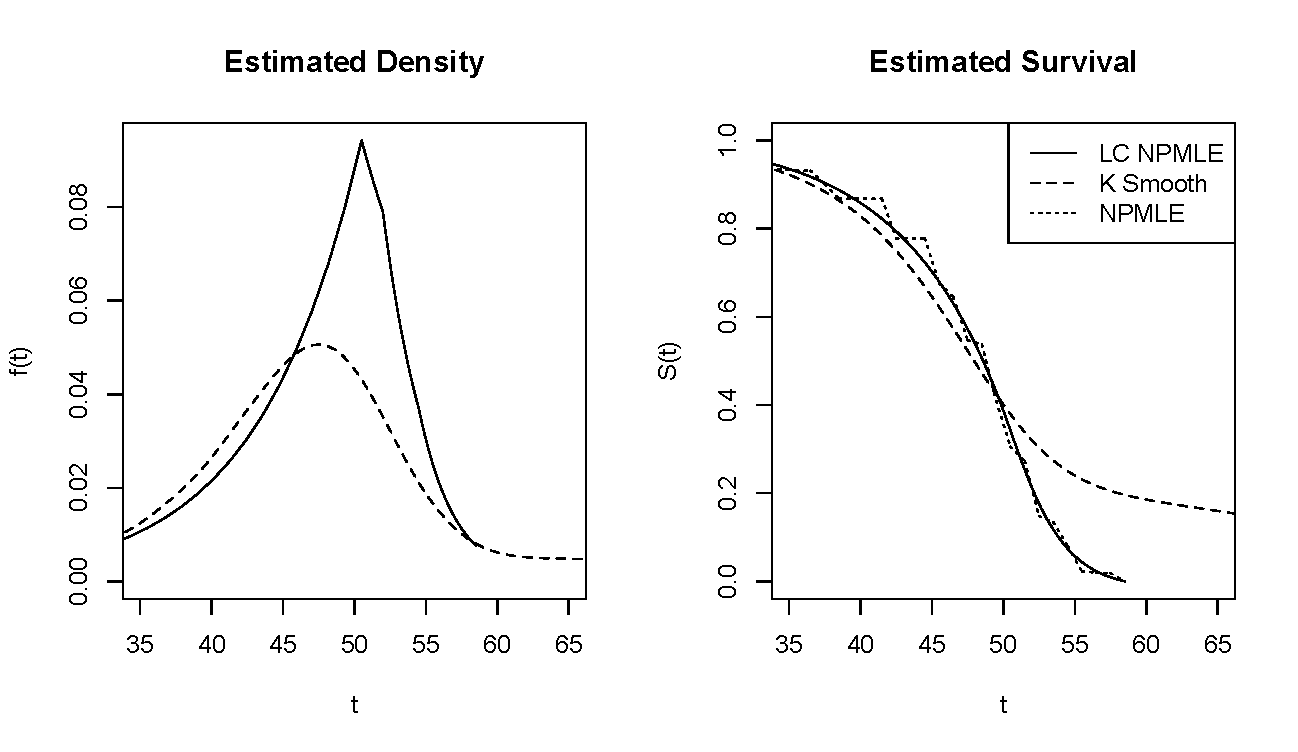
\includegraphics[width = 12cm]{MenoPlot.pdf}}
\caption{Estimated Functions}
\end{figure}		
	
	Plotted estimates can be seen in figure 4 for the menopause data. The full estimator is not shown, in order to be able to see the estimator in better detail. The full estimator can been in figure 5 in the appendix. A few key features we see is that the log concave NPMLE has a much more jagged density estimator than the kernel smoother. This can be seen as a disadvantage for the log concave NPMLE where smoothness is a priority. Also, we note that the kernel smoother and log concave NPMLE disagree with each other very heavily, especially on the tail. The log concave NPMLE places 0 masses beyond t = 58.5, while the kernel smoother places mass as far as t = 100. Examining the estimated survival curves, we note that the log concave NPMLE appears to agree with the unconstrained NPMLE. Also, the NPMLEs appear to agree with what is known about menopause, while the kernel smoother appears to be a less accurate portrayal of the distribution of time to menopause. For example, Treloar 1981 presents data from a longitudinal study. Excluding the cases lost to follow up, all 729 cases had experienced menopause by age 59 (and only one had experienced menopause after 58). However, the kernel smoother estimates that $S(59) =  0.19$. In contrast, both the log concave NPMLE and unconstrained NPMLE place 0 mass beyond 58.5, which agree much better with Treloar's findings. The current implementation of the LC NPMLE algorithm took 2.42 seconds to converge, although it is very important to note that this the best case scenario (see appendix on acceleration from ties). In contrast, the kernel smoother took 16.5 seconds and the unconstrained NPMLE algorithm, as implemented in the CRAN package  MLEcens, took 0.139 seconds to converge. 
	
	
	{\section{Simulations} } 
	
	Now that a reasonably fast algorithm has been created for computing the log concave NPMLE, the finite sample size operating characteristics can be examined and compared to the competing estimators. In order to examine which estimator performed best in estimating quantiles, the bias and standard deviation of the estimated 0.1, 0.25, 0.5, 0.75 and 0.9 quantiles were compared across the estimators. 
			
	The data was simulated across a variety of different situations. For most of the simulations, current status data was used, as this simplified the process of censoring. The true time $T$ was simulated along with the censoring time $C$. For simplicity, $C$ followed the same distribution as $T$. The only information kept was $C$ and whether the event was right or left censored. If $T_i$ was right censored, $R_i$ was set to the maximum value of $C \times 1.1$.

	A variety of different distributions were used to examine how the estimators worked in different scenarios. The distributions tested were gamma(shape = 2, rate = 2), gamma(shape = 100, rate = 2), weibull(shape = 6, scale = 4),  lognormal($\mu = 0$, $\sigma = 1$) and a gamma mixture with p = (0.5, 0.5), component 1 = gamma(shape = 2, rate = 2), component 2 = gamma(shape = 5, rate = 1). It should be noted that the last two simulations violate the assumption of log concavity; the log normal distribution is mildly non log concave due to heavy tails, while the gamma mixture model is heavily non log concave due to bimodality. In each of the simulations, datasets were generated with $n$ = 50, 200 and 800. For $n$ = 50 and 200, MC = 400 simulations were generated. For $n$ = 800, MC = 100 simulations were generated.
	
	Tables of the results are given in the appendix. Some general trends that were noted from the simulations were:
	
\vspace{3mm}	
	
\begin{itemize}	
		
	\item For log concave data, the log concave NPMLE always outperforms the unconstrained NPMLE in both bias and standard deviation.
			
	\item For log concave data, the log concave NPMLE occasionally displays higher standard deviation than the kernel smoother, especially in the lower tails of the smaller samples. However, the kernel smoother often has heavier bias in the upper tail. This bias tends to \emph{increase} as $n$ increases.
	
	\item The kernel smoother shows very heavy bias when the censored intervals cover vast regions where the density is very close to 0, such as the gamma (100,2) case. Again, this bias from the kernel smoother appears to increase as $n$ increases. This bias is thought to be the cause of the discrepancy in estimates for the motivating example. 
	
	\item For log concave data, the bias approaches 0 fairly quickly. For samples over 200, the largest bias to standard deviation ratio was 0.4, although for $n$ = 50, we observe a bias to standard deviation ratio of 0.7. 
	
	\item The standard deviation appears to be shrinking close to the typical $n^{1/2}$ rate for the log concave NPMLE. The unconstrained NPMLE standard deviation appears to be reducing close to the theoretic rate of $n^{1/3}$. The rate of convergence for kernel smoother varied wildly. For distributions where the bias was minimal, such as the gamma(2,2), the standard deviation appeared to shrink at the $n^{1/2}$ rate. However, it appeared to do much worse when it suffered from bias, such as the gamma (100,2) case.

	\item For log normal data, significant bias was observed in the estimation of the upper tail for the log concave NPMLE. While this bias reduced as $n$ increased, it did not appear to converge to 0. While the unconstrained NPMLE showed significant bias in small samples, the bias appeared to converge to 0. The kernel smoother observed heavier bias than the log concave NPMLE in estimating all cases except estimating the 0.9 quartile with $n$ = 50. 
		
	\item For mixture gamma data, significant bias was observed for almost all quantiles for the log concave NPMLE, although this was about equal for the kernel smoother. While the unconstrained NPMLE suffered from significant bias in $n$ = 50, by $n = 200$, these biases were mostly insiginificant.
		
	\item For density estimation, the trend was very consistent; the log concave NPMLE displayed lower bias but higher standard deviation than the kernel smoother. The bias from the kernel smoother was often substantial. This bias often did not decrease with an increase in sample size. 
	
	\item While the log concave NPMLE did well in terms of bias, the standard deviation was often so high that it would be unreasonable to use for density estimation without large data sets ($n \geq 800$) 

\end{itemize}	

	From these results, we would conclude that the log concave NPMLE would be the estimator of choice for quantile estimation with current status data that was believed to be log concave. The advantage of the log concave estimator increases as $n$ increases. In large data sets, the log concave NPMLE may be reasonable for density estimation, but it is not recommended for smaller data sets ($n \leq 400$).
	
	{\section{Future Work} } 

	Uniqueness of the solution has not been shown yet. In the case of the log concave NPMLE for exact data, uniqueness is shown using the fact that the log likelihood is strictly convex (Rufibach 2007). However, in the case of interval censored data, we know that the log likelihood is not strictly convex and in fact have shown that local maximum, which are less than the global maximum, exist. In the case of the univariate unconstrained NPMLE, it has been shown that the solution does not have mixture non-uniqueness (for a solution set of intervals, there is only one assignment of mass to each interval which maximizes the likelihood function) but does suffer from representational non-uniqueness (for a mixed mass and interval, any assignment of mass within the interval leads to the same likelihood) (Gentleman and Vandal 2001). The proof although it depends on the fact that the solution only assigns mass to the Turnbull intervals. 
	
	There are several trivial example of representational non-uniqueness for the log concave NPMLE, although it is very easy to show that it must have much less of an affect on the log concave NPMLE than on the constrained NPMLE. This is because representational non-uniqueness can only occur in contribution intervals with active points, as $\hat \phi(x)$ will be strictly linear in intervals that do not contain an active point. It is not clear whether $\hat \phi(x)$ could have mixture non-uniqueness; the proof of that the unconstrained NPMLE does have mixture non-uniqueness requires the fact mass will only be assigned to maximal intersections, which is not true for the log concave NPMLE. To investigate whether mixture non-uniqueness could be an issue, the algorithm was run several times from random initial values but always found to converge to the same solution for each simulated data set, suggesting that mixture non-uniqueness may not occur for the log concave NPMLE. However, no theoretic proof of this exists at this time.
	
	Although the algorithm presented in this paper is acceptable for small to moderate sized data sets or larger data sets with large amounts of ties (see appendix), it would be too slow for larger data sets with large numbers of unique values. For example, simulated data sets with no rounding of the data showed that for case II interval censored data, the algorithm took on average 4 seconds for n = 200, 8.5 seconds for n = 300 and 19 seconds for n = 400. Considering that several inference techniques, such as bootstrapping, require recalculating of the estimate, this would be too slow for larger datasets. In contrast, the MLEcens CRAN package can compute the unconstrained NPMLE for n = 400 in around 0.05 seconds. 
	
	In the appendix, it is noted that the algorithm can find local maximum, returning an estimate which can differ significantly from the true MLE on the tails. While an ad hoc fix is presented, it would be preferable to find a transformation of $\phi(x)$ such that the estimate could step away from the local max and toward the global max. Such a step would likely have to be consider both the length of the tails of $\phi(x)$ and the log density of the tails of $\phi(x)$ simultaneously. Adding such a step would likely both accelerate the algorithm and help insure convergence to the global maximum.  
	
	It is worth noting that we are calculating an approximation of the log concave NPMLE, due to the fact that we do not know the exact location of $m_k$ for the $k^{th}$ interval. While it would not be very difficult to adjust the algorithm to find $m_k$, it was speculated that this would be relatively computationally expensive and the difference made in the estimator would be undetectable.  However, it may be more theoretically pleasing to know the estimator is the true log concave NPMLE. Perhaps there is a parameterization such that $m_k$ (instead of just $mid_k$) is included in the set of knots considered, at a low computation cost.
	
	Now that an algorithm has been developed which can handle moderate sized data sets, several important questions about the operating characteristics of the LC NPMLE must be addressed. Two topics unique to this estimator are that must be addressed is assessing the bias resulting from violation of the logconcave assumption and creating a test of log concavity. We present two potential methods of testing the log concavity assumption. The first would involve computing the integrated squared difference between the unconstrained NPMLE and the logconcave NPMLE survival function. In order to sample from the null distribution, censored samples can be taken from the log concave NPMLE estimated distribution and the unconstrained and log concave NPMLEs can be estimated. A second approach could be a likelihood ratio test, in which the maximum log concave likelihood would be compared to the maximum unconstrained likelihood. Because the solution would be on the boundary, the distribution of the test statistic under the null hypothesis is not trivial. More work is required to assess the validity of these tests.  

{\section{Appendix} } 

%	{\subsection{Stopping Criterion and Active Point Selection} }

%	KKT conditions (Kuhn and Tucker 1951) were used both for the stopping criterion and selection of new active points. However, using the $\phi$ parameterization is very unstable for a stopping criterion and is very ineffective as a method for picking new active points. Instead, it is helpful to examine the derivatives in terms of $\Delta^2 \phi_k = \phi'(x_k)_{(-)} - \phi'(x_k)_{(+)}$, i.e., the change in the slope of $\phi(x)$ at $x_k$. The restriction of log concavity implies $\Delta^2 \phi_k \le 0$. The knot at $x_k$ is active if $\Delta^2 \phi_k < 0$ and inactive if $\Delta^2 \phi_k = 0$. The knot $i$ such that $i = argmin\left( \frac {dl}{d\Delta^2 \phi_i} \right)$ is selected as the next active point. 
	
%	Let $a$ be the set of indices such that $x_a$ is an active point and $na$ be the set of indices such that $x_{na}$ are inactive. Define $err = max \left(  - \frac {dl}{d\Delta^2 \phi_{na}} \cup \left| \frac {dl}{d\Delta^2 \phi_a} \right| \right)$. The algorithm converges when $err < \epsilon$, for some $\epsilon$. In all the examples used in this paper, $\epsilon = 10^{-5}$ was used. 
	
	{\subsection{Simulation Results} }
	
	{\subsubsection{Quantile Estimation} } 
	
		The tables below give the results of the simulation for quantile estimation. The top of the table shows the 0.1, 0.25, 0.5, 0.75 and 0.9 quantile, respectively, of the distribution of the simulated data. The main table shows the bias and standard deviation found for each of the estimators, organized by sample size. LC = log concave NPMLE, UC = unconstrained NPMLE and KS = Kern Smoother.
	

\begin{center}	

\begin{table}[H]

\caption{Quantile Estimation for Gamma(2, 2)}

\begin{tabular} {| c | c | c | c | c | c | c | } 


	 \hline
		&Q(p)&	0.27 (0.1)&	0.48 (0.25)&	0.84 (0.5)&	1.35 (0.75)&	1.94 (0.9)\\ 
 \hline 
 	$n$ & & \multicolumn{5}{|c|}{Bias / Standard Deviation} 
 \\ 
 \hline 
\multirow{3}{*}{50}		&	LC	&-0.04/0.11	&-0.04/0.11	&-0.04/0.14	&0.01/0.22	&0.21/0.31\\ 
			&	UC	&-0.11/0.14	&-0.07/0.17	&-0.05/0.22	&0.02/0.33	&0.27/0.4\\ 
			&	KS	&0.03/0.07	&-0.03/0.09	&-0.07/0.13	&-0.1/0.24	&-0.11/0.37\\ 
	\hline 
\multirow{3}{*}{200}		&	LC	&-0.01/0.07	&-0.01/0.06	&-0.02/0.08	&-0.01/0.13	&0.07/0.21\\ 
			&	UC	&-0.05/0.09	&-0.02/0.12	&-0.03/0.14	&0/0.22	&0.12/0.35\\ 
			&	KS	&0.02/0.04	&-0.01/0.05	&-0.02/0.07	&-0.05/0.14	&-0.28/0.35\\ 
	\hline 
\multirow{3}{*}{800}		&	LC	&0/0.03	&0/0.03	&-0.01/0.04	&-0.01/0.06	&0.03/0.11\\ 
			&	UC	&0/0.05	&-0.02/0.06	&-0.01/0.08	&0.01/0.14	&0.05/0.21\\ 
			&	KS	&0.01/0.02	&0/0.02	&0/0.04	&-0.02/0.07	&-0.47/0.29\\ 
	\hline 

\end{tabular}

\end{table}


\begin{table}[H]

\caption{Quantile Estimation Gamma(100, 2)}

\begin{tabular} {| c | c | c | c | c | c | c | } 

	 \hline
		&Q(p)&	43.7 (0.1)&	46.5 (0.25)&	49.8 (0.5)&	53.3 (0.75)&	56.5 (0.9)\\ 
 \hline 
 	$n$ & & \multicolumn{5}{|c|}{Bias / Standard Deviation} 
 \\ 
 \hline 
\multirow{3}{*}{50}		&	LC	&-0.4/2.55	&-0.08/1.54	&-0.05/1.14	&0.06/1.44	&0.72/2.14\\ 
			&	UC	&-0.67/3.73	&-0.23/2.08	&-0.21/1.75	&0.03/2.03	&0.93/2.41\\ 
			&	KS	&11.48/7.22	&3.36/3.15	&-0.1/1.51	&-2.24/1.56	&-3.89/1.92\\ 
	\hline 
\multirow{3}{*}{200}		&	LC	&-0.1/1.13	&0.08/0.73	&-0.02/0.67	&-0.1/0.81	&0.18/1.19\\ 
			&	UC	&-0.17/1.51	&0.04/1.1	&-0.11/1.06	&-0.01/1.23	&0.14/1.82\\ 
			&	KS	&12.64/5.73	&1.88/1.33	&-0.22/0.67	&-1.69/0.93	&-3.83/1.6\\ 
	\hline 
\multirow{3}{*}{800}		&	LC	&0.14/0.68	&0.04/0.44	&-0.07/0.33	&-0.12/0.44	&0/0.61\\ 
			&	UC	&0.1/0.97	&-0.03/0.64	&-0.1/0.51	&-0.05/0.75	&-0.04/0.98\\ 
			&	KS	&15.94/3.23	&1.18/0.66	&-0.25/0.3	&-1.22/0.48	&-4.57/1.35\\ 
	\hline 

\end{tabular}

\end{table}

\begin{table}[H]

\caption{Quantile Estimation for Weibull(6, 4)}

\begin{tabular} {| c | c | c | c | c | c | c | } 

	 \hline
		&Q(p)&	2.75 (0.1)&	3.25 (0.25)&	3.76 (0.5)&	4.22 (0.75)&	4.6 (0.9)\\ 
 \hline 
 	$n$ & & \multicolumn{5}{|c|}{Bias / Standard Deviation} 
 \\ 
 \hline 
\multirow{3}{*}{50}		&	LC	&-0.12/0.33	&-0.02/0.21	&0/0.15	&0.01/0.18	&0.06/0.25\\ 
			&	UC	&-0.24/0.38	&-0.09/0.29	&-0.03/0.23	&0.05/0.24	&0.17/0.26\\ 
			&	KS	&0.5/0.44	&0.19/0.26	&0.01/0.16	&-0.13/0.17	&-0.25/0.19\\ 
	\hline 
\multirow{3}{*}{200}		&	LC	&-0.03/0.18	&0.01/0.12	&0/0.09	&0/0.09	&0.02/0.14\\ 
			&	UC	&-0.1/0.25	&-0.05/0.2	&-0.02/0.16	&0.02/0.15	&0.08/0.19\\ 
			&	KS	&0.51/0.31	&0.12/0.14	&0.01/0.09	&-0.09/0.1	&-0.25/0.14\\ 
	\hline 
\multirow{3}{*}{800}		&	LC	&0/0.11	&0.01/0.06	&0/0.05	&-0.01/0.05	&0/0.07\\ 
			&	UC	&-0.03/0.19	&-0.01/0.12	&-0.02/0.11	&0/0.1	&0.02/0.12\\ 
			&	KS	&0.55/0.17	&0.08/0.06	&0/0.04	&-0.07/0.05	&-0.3/0.1\\ 
	\hline 

\end{tabular}

\end{table}

\begin{table}[H]

\caption{Quantile Estimation for Lognormal(0, 1)}
  
\begin{tabular} {| c | c | c | c | c | c | c | } 

	 \hline
		&Q(p)&	0.28 (0.1)&	0.51 (0.25)&	1 (0.5)&	1.96 (0.75)&	3.6 (0.9)\\ 
 \hline 
 	$n$ & & \multicolumn{5}{|c|}{Bias / Standard Deviation} 
 \\ 
 \hline 
\multirow{3}{*}{50}		&	LC	&-0.04/0.13	&-0.09/0.15	&-0.14/0.23	&0.02/0.43	&0.77/0.73\\ 
			&	UC	&-0.12/0.17	&-0.11/0.23	&-0.12/0.4	&-0.04/0.94	&0.59/1.95\\ 
			&	KS	&0.18/0.21	&-0.11/0.13	&-0.35/0.29	&-0.49/0.7	&-0.54/1.56\\ 
	\hline 
\multirow{3}{*}{200}		&	LC	&0/0.07	&-0.03/0.07	&-0.08/0.12	&-0.02/0.25	&0.49/0.46\\ 
			&	UC	&-0.05/0.09	&-0.03/0.13	&-0.07/0.24	&-0.01/0.5	&0.27/1.05\\ 
			&	KS	&0.16/0.16	&-0.08/0.07	&-0.26/0.18	&-0.28/0.37	&-0.58/1.09\\ 
	\hline 
\multirow{3}{*}{800}		&	LC	&0/0.03	&-0.02/0.03	&-0.07/0.06	&-0.04/0.12	&0.39/0.22\\ 
			&	UC	&-0.03/0.06	&-0.03/0.07	&0/0.14	&-0.04/0.33	&0.08/0.83\\ 
			&	KS	&0.1/0.06	&-0.08/0.03	&-0.19/0.11	&-0.13/0.18	&-0.78/0.91\\ 
	\hline 

\end{tabular}

\end{table}

\begin{table}[H]

\caption{Quantile Estimation for Gamma Mixture}

\begin{tabular} {| c | c | c | c | c | c | c | } 

	 \hline
		&Q(p)&	0.41 (0.1)&	0.84 (0.25)&	2.17 (0.5)&	4.68 (0.75)&	6.72 (0.9)\\ 
 \hline 
 	$n$ & & \multicolumn{5}{|c|}{Bias / Standard Deviation} 
 \\ 
 \hline 
\multirow{3}{*}{50}		&	LC	&-0.14/0.22	&-0.36/0.31	&-0.27/0.53	&0.51/0.79	&0.95/1.03\\ 
			&	UC	&-0.26/0.33	&-0.28/0.57	&-0.3/1.02	&0.17/1.31	&0.96/1.43\\ 
			&	KS	&-0.02/0.21	&-0.42/0.28	&-0.43/0.51	&0.09/0.9	&0.01/1.26\\ 
	\hline 
\multirow{3}{*}{200}		&	LC	&-0.03/0.11	&-0.21/0.14	&-0.14/0.27	&0.39/0.43	&0.32/0.63\\ 
			&	UC	&-0.09/0.18	&-0.09/0.3	&-0.2/0.77	&0.07/0.89	&0.43/1.09\\ 
			&	KS	&-0.04/0.09	&-0.28/0.13	&-0.15/0.26	&0.23/0.53	&-0.51/1.01\\ 
	\hline 
\multirow{3}{*}{800}		&	LC	&0.01/0.05	&-0.15/0.07	&-0.08/0.13	&0.38/0.22	&0.04/0.35\\ 
			&	UC	&-0.05/0.11	&-0.05/0.15	&-0.04/0.45	&0.04/0.53	&0.07/0.79\\ 
			&	KS	&-0.05/0.04	&-0.18/0.06	&0.03/0.14	&0.31/0.26	&-0.97/0.64\\ 
	\hline 

\end{tabular}

\end{table}
	
\end{center}
	
	{\subsubsection{Density Estimation} } 
	
	The tables below give the results of the simulation for density estimation at the quantiles. The top of the table shows the density of the simulated data at the  0.1, 0.25, 0.5, 0.75 and 0.9 quantiles. The main table shows the bias and standard deviation found for each of the estimators, organized by sample size. LC = log concave NPMLE and KS = Kern Smoother. The unconstrained NPMLE is excluded as it does not provide density estimates. 

	
\begin{center}	
	
\begin{table}[H]

\caption{Density Estimation at Quantiles for Gamma (2,2) }
	
\begin{tabular} {| c | c | c | c | c | c | c | } 

	 \hline
		&f(p)&	0.62(0.1)&	0.74(0.25)&	0.63(0.5)&	0.36(0.75)&	0.16(0.9)\\ 
 \hline 
 	$n$ & & \multicolumn{5}{|c|}{Bias / Standard Deviation} 
 \\ 
 \hline 
\multirow{3}{*}{50}		&	LC	&0.11/0.35	&-0.01/0.31	&-0.04/0.21	&-0.09/0.22	&0.01/0.13\\ 
			&	KS	&0.15/0.1	&0.12/0.11	&0.01/0.1	&-0.02/0.08	&-0.02/0.07\\ 
	\hline 
\multirow{3}{*}{200}		&	LC	&-0.05/0.27	&0/0.15	&0/0.11	&-0.03/0.08	&-0.02/0.09\\ 
			&	KS	&0.09/0.08	&0.05/0.07	&-0.01/0.08	&0.02/0.05	&0.02/0.03\\ 
	\hline 
\multirow{3}{*}{800}		&	LC	&-0.05/0.12	&0.01/0.09	&0.01/0.07	&-0.01/0.04	&-0.02/0.04\\ 
			&	KS	&0.05/0.04	&0.01/0.04	&-0.01/0.04	&0.05/0.03	&0.05/0.02\\ 
	\hline 

\end{tabular}
	
\end{table}	
	
	
\begin{table}[H]

\caption{Density Estimation at Quantiles for Gamma(100,2)}

\begin{tabular} {| c | c | c | c | c | c | c | } 

	 \hline
		&f(p)&	.038(0.1)&	.067(0.25)&	.08(0.5)&	.061(0.75)&	.032(0.9)\\ 
 \hline 
 	$n$ & & \multicolumn{5}{|c|}{Bias / Standard Deviation} 
 \\ 
 \hline 
\multirow{3}{*}{50}		&	LC	&.007/.029	&-.007/.036	&-.003/.029	&-.006/.034	&.003/.026\\ 
			&	KS	&.01/.005	&.027/.007	&.032/.008	&.016/.007	&-.003/.006\\ 
	\hline 
\multirow{3}{*}{200}		&	LC	&-.004/.022	&-.002/.018	&.003/.016	&-.002/.015	&-.006/.018\\ 
			&	KS	&.012/.003	&.023/.005	&.023/.007	&.012/.005	&0/.004\\ 
	\hline 
\multirow{3}{*}{800}		&	LC	&-.002/.01	&.003/.009	&0/.013	&-.001/.009	&-.004/.009\\ 
			&	KS	&.017/.002	&.022/.003	&.014/.006	&.01/.004	&.005/.002\\ 
	\hline 

\end{tabular}
\end{table}
	
	
\begin{table}[H]

\caption{Density Estimation at Quantiles for Weibull(6,4)}
\begin{tabular} {| c | c | c | c | c | c | c | } 

	 \hline
		&f(p)&	0.21(0.1)&	0.4(0.25)&	0.55(0.5)&	0.49(0.75)&	0.3(0.9)\\ 
 \hline 
 	$n$ & & \multicolumn{5}{|c|}{Bias / Standard Deviation} 
 \\ 
 \hline 
\multirow{3}{*}{50}		&	LC	&0.02/0.16	&-0.05/0.23	&-0.02/0.19	&-0.04/0.27	&0.02/0.23\\ 
			&	KS	&0.02/0.04	&0.07/0.07	&0.11/0.09	&0.09/0.07	&0/0.06\\ 
	\hline 
\multirow{3}{*}{200}		&	LC	&-0.04/0.11	&-0.01/0.09	&0.01/0.1	&-0.02/0.13	&-0.03/0.17\\ 
			&	KS	&0.04/0.03	&0.06/0.05	&0.08/0.06	&0.08/0.05	&0.03/0.04\\ 
	\hline 
\multirow{3}{*}{800}		&	LC	&-0.01/0.05	&0/0.06	&0.01/0.07	&0/0.08	&-0.03/0.08\\ 
			&	KS	&0.05/0.02	&0.06/0.03	&0.05/0.04	&0.08/0.03	&0.06/0.02\\ 
	\hline 

\end{tabular}

\end{table}	

\begin{table}[H]

\caption{Density Estimation at Quantiles for Lognormal(0,1)}

\begin{tabular} {| c | c | c | c | c | c | c | } 

	 \hline
		&f(p)&	0.63(0.1)&	0.62(0.25)&	0.4(0.5)&	0.16(0.75)&	0.05(0.9)\\ 
 \hline 
 	$n$ & & \multicolumn{5}{|c|}{Bias / Standard Deviation} 
 \\ 
 \hline 
\multirow{3}{*}{50}		&	LC	&0.17/0.28	&0.06/0.21	&-0.04/0.12	&-0.06/0.09	&0/0.04\\ 
			&	KS	&0.35/0.07	&0.28/0.09	&0.03/0.08	&-0.05/0.04	&-0.01/0.03\\ 
	\hline 
\multirow{3}{*}{200}		&	LC	&0.03/0.16	&0.07/0.09	&0/0.05	&-0.04/0.03	&-0.01/0.02\\ 
			&	KS	&0.32/0.06	&0.25/0.08	&0.01/0.06	&-0.05/0.03	&0/0.02\\ 
	\hline 
\multirow{3}{*}{800}		&	LC	&0.02/0.08	&0.06/0.05	&0.01/0.02	&-0.03/0.01	&-0.01/0.01\\ 
			&	KS	&0.29/0.05	&0.21/0.07	&-0.02/0.04	&-0.04/0.03	&0.01/0.01\\ 
	\hline 

\end{tabular}

\end{table}

\begin{table}[H]
\caption{Density Estimation at Quantiles for Gamma Mixture}

\begin{tabular} {| c | c | c | c | c | c | c | } 

	 \hline
		&f(p)&	0.36(0.1)&	0.32(0.25)&	0.11(0.5)&	0.09(0.75)&	0.05(0.9)\\ 
 \hline 
 	$n$ & & \multicolumn{5}{|c|}{Bias / Standard Deviation} 
 \\ 
 \hline 
\multirow{3}{*}{50}		&	LC	&0.13/0.11	&0.08/0.08	&-0.07/0.04	&-0.01/0.04	&0.01/0.03\\ 
			&	KS	&0.21/0.03	&0.13/0.04	&-0.07/0.03	&0.01/0.02	&0.01/0.02\\ 
	\hline 
\multirow{3}{*}{200}		&	LC	&0.09/0.05	&0.07/0.03	&-0.06/0.01	&0.01/0.01	&0.01/0.01\\ 
			&	KS	&0.18/0.03	&0.08/0.03	&-0.07/0.02	&0.02/0.02	&0.01/0.01\\ 
	\hline 
\multirow{3}{*}{800}		&	LC	&0.08/0.02	&0.07/0.02	&-0.06/0.01	&0.01/0.01	&0.01/0.01\\ 
			&	KS	&0.13/0.02	&0.04/0.02	&-0.05/0.01	&0.02/0.01	&0.02/0\\ 
	\hline 

\end{tabular}
\end{table}
	
\end{center}
	
	{\subsection{Efficient Likelihood Functions} } 	
	
	For this algorithm, efficient calculation of the likelihood and derivatives is paramount for an efficient algorithm. The first step in calculating the likelihood function is calculating a vector {\bf p} in which $p_k = \int_{t_k}^{t_{k+1}} e^ { \phi(x) } \,dx$, or the mass placed within the $k^{th}$ contribution interval. Because $\phi(x)$ is linear between the knots, the solution is in closed form. Define $\phi(t_k) = \phi_k$ and $\Delta x_k = x_{k+1} - x_k$. Integrating gives us 
	
	\[ p_k = \frac{\Delta t_k} {\Delta \phi_k } \times (e^{\phi_{k+1} } - e^{\phi_k } ) 
	\]
	
	This is undefined if $\phi_{k+1} = \phi_k$ and so the limit as $\phi_{k+1} \rightarrow \phi_k$ will be used instead. The limit is $e^{\phi_k} \times \Delta t_k$. It was also observed that calculating $p_k$ suffers from numeric instability as $\phi_k \rightarrow \phi_{k+1}$. In order to deal with, if $|\Delta\phi_k | < 10^{-5}$, $p_k$ will be replaced with a first order Taylor approximation, i.e., 
	
	\[ p_k \approx e^{\phi_k} \times \Delta t_k + \frac{dp_k}{d\phi_{k+1}} \times \Delta \phi_k 
	\]
	\[
	= e^{\phi_k} \times \Delta t_k + e^{\phi_k} \times \frac {\Delta t_k} {2} \times \Delta \phi_k
	\]
	\[
	= e^{\phi_k} \times \Delta t_k \times \left(1 + \frac{\Delta \phi_k}{2} \right)
	\]
	
	Once {\bf p} has been calculated, the likelihood function can be calculated similar to the unconstrained NPMLE. This will require a matrix $M$, in which the $i, j^{th}$ entry is an indicator for whether the $i^{th}$ contribution interval is within the $j^{th}$ observational interval. Then the likelihood function can be calculated by
	\[ \displaystyle \sum_{i = 1}^n \log \left( \int_{L_i}^{R_i} e^ { \phi(x) } \,dx \right) - n \times \log \left(  \int_{-\infty}^{\infty} e^ { \phi(x) } \,dx \right) 
	\]
	\[=  \displaystyle \sum_{i = 1}^n \log \left({\bf p} M \right) - n \times \log \left( \sum_{i = 1}^{k} {\bf p} \right) 
	\]
	
	Similar methods were used calculate the derivative vectors.
	
		{\subsection{Fixing the Tails} }
	
	When computing the log concave NPMLE with exact observations, the area which must have positive mass is known in advance (i.e. the range of all observed times). When computing the log concave NPMLE for interval censored data, this not the case. There will be several contribution intervals which receive 0 mass at the log concave NPMLE. A trivial example is to consider if the data consisted of two overlapping intervals. The log concave NPMLE would place all the mass in the overlap and no mass to the other two surrounding contribution intervals. In the case of the unconstrained NPMLE, the mass was known to be positive only in the set of Turnbull intervals. However, the log concave constraint implies that this is not the case and often some of the contribution intervals outside of the minimum and maximum Turnbull intervals will receive positive mass at the log concave NPMLE, while others will not.
	 		
	Because of this, simply allowing the earlier steps to find the log densities	 at the tails of the estimated density can lead to numerical instability as $\phi(x) \rightarrow -\infty$. Numerical instability typically happened in the range of $\phi(x) = -1000$ for some $x$, as derivatives and second derivatives approached 0. Along with numerical issues is computational cost issues. Consider that if $\phi(x) = -10$ for some $x$, then the density is $4.5 \times 10^{-5}$ times the density at the mode, indicating $\phi(x)$ is very likely $-\infty$ at $\hat \phi(x)$. Even if numerical issues were not observed, allowing the algorithm to meet the stopping criterion can be very computationally expensive for a rather trivial transformation of $\phi(x)$. 
	
	To cope with this, it was periodically checked if setting $\phi(x)$ to $-\infty$ increases the likelihood for $x$ on the tails if $\phi(x) < -t$ for some threshold $t$. Interestingly, choosing $t$ too small leads to local maxes which can be considerably less than the global max, even if optimization techniques are used to check if adding mass back to the tails which have been set to $-\infty$. For poorly chosen $t$, such as $t = 1$, the difference in log likelihood was observed to be as high as 1.5 and the mass could be significantly different on the tails, despite the convergence criterion being satisfied. On the other hand, setting very large $t$, such as 500, was found to increase the number of iterations required several fold. Fortunately, there appears to be a large region for choices of $t$ such that neither issues occurred. The performance across $t$ = 1, 5, 10, 20 and 40 was examined. While it was found that $t = 10$ appeared satisfactory, for robustness $t = 20$ was selected as it lead to a small increase in average iterations (about 15\% more). With this fix, it was found that even with random starting values, the algorithm lead to the same estimate. 
	
	It should be noted that even with this fix, it is theoretically possible that the algorithm could prematurely set $\phi(x_0)$ to $-\infty$ when $\phi(x_0)$ should have positive density at the log concave NPMLE. Fortunately, it was observed that while these mistakes can have a substantial effect on the likelihood, the estimates themselves are fairly similar except on the tails of $\phi(x)$. Thus, while this algorithm potentially may converge without finding the true maximum likelihood, the estimate found should be very close to the true estimate. 
			

	
	{\subsection{Acceleration from Ties} } 
	
	It should be noted that in calculating the likelihood and derivatives, the most computationally expensive step is the multiplication of $ {\bf p}M $. The length of {\bf p} is $K-1$ and the dimensions of $M$ are $(K-1) \times n$. Thus, the computation time is heavily reliant on $K$. The theorem presented in this paper dictates that the maximum length of $K$ is $4n - 1$. Fortunately, when there are ties in the data, many of these knots will be repetitive and $K$ may be significantly smaller. In fact, the number of knots required is at most $2U - 1$, where $U$ is the number of unique times in the data set. For example, in the motivating example, $n = 2,423$, but the number of unique times observed was 102 (age was rounded to the half year). Therefore, the number of knots used was 203, instead of 9,691. Thus, without modifying the algorithm, the LC NPMLE was calculated in approximately 17 seconds. In contrast, if all the times in the data were unique, the algorithm would take about 20 seconds to converge for a data set of size $n = 350$. It is worth noting that almost all the datasets that appear frequently in the literature have a large number of ties in the data.
	
	In the case of current status data, ties in the data can be used to further accelerate the calculation of ${\bf p} M$. With current status data, for each observation, either $L_i = 0$ or $R_i = \infty$. Thus, if the times are rounded, there is a high probability that the data set will contain a large number of observations such that $L_i = L_j$ and $R_i = R_j$. Define $M.r$ = $M$, but removing any redundant columns (i.e. observations that contain the exact same times). Define {\bf w} to be a vector s.t. $w_i =$ number of times the set of the $i^{th}$ unique set of times appears in the data set. Then while $M$ is $(K-1) \times n$, $M.r$ is at most $(K-1) \times (2U - 2)$. It should be noted that
	
	\[ {\bf p} M = {\bf p} M.r \cdot {\bf w}
	\] 

	Applying this to the motivating example, the computation time was reduced from 17 seconds to 1.54 seconds. 

\begin{figure}[h]
\centerline{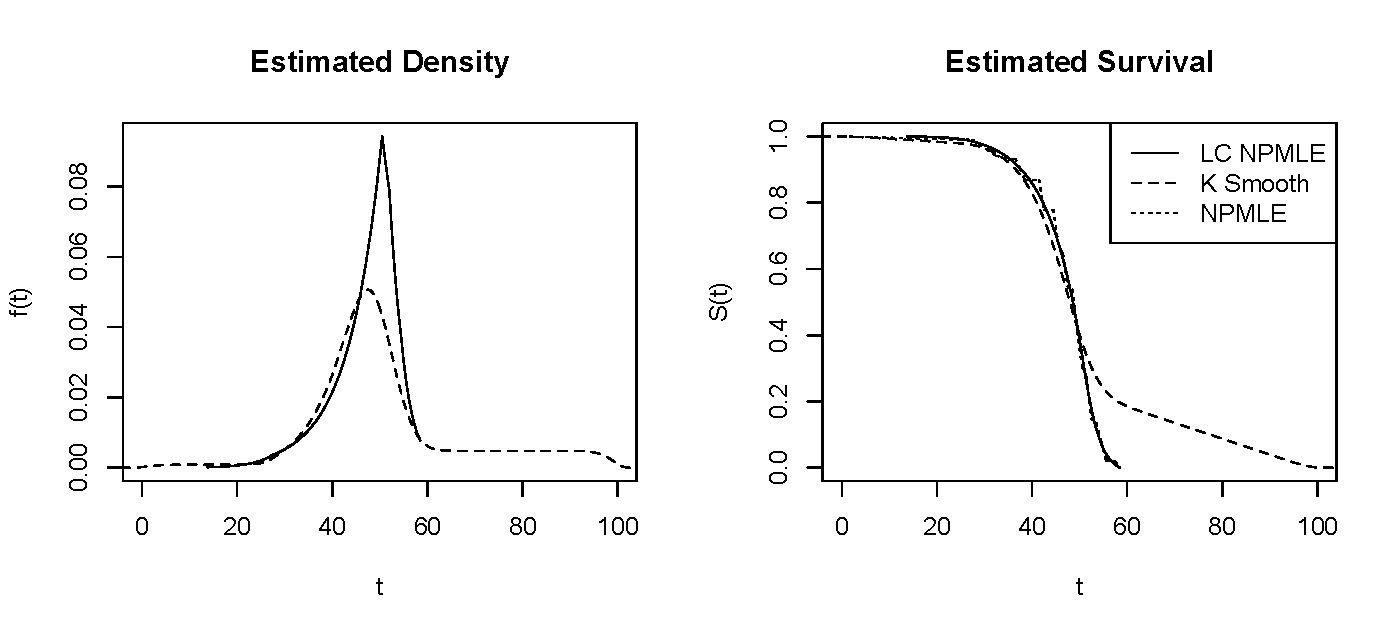
\includegraphics[width = 10cm]{FullMenoPlot.pdf}}
\caption{Estimated Functions}
\end{figure}		




	
{\section{References} }

Bagnoli, M., Bergstorm, T., (2005), Log-concave Probability and its Applications, \emph{Economic Theory} Vol 26 No. 2, 445-469

\vspace{3mm}

Betensky, R., Lindsey, J., Ryan, L., Wand, M. (1999), Local EM Estimation of the Hazard Function Interval-Censored Data, \emph{Biometrics} Vol 55 238-245

\vspace{3mm}

Braun, J., Duchense, T., Stafford, J. (2005): Local Likelihood Density Estimation for Interval Censored Data, \emph{The Canadian Journal of Statistics}, Vol 33 No.1, 39-60

\vspace{3mm}

Chang, G., Walther, G. (2007): Clustering with Mixtures of Log-Concave Distributions, \emph{Computational Statistics and Data Analysis}, Vol 51, No. 12, 6242-6251

\vspace{3mm}

D\"umbgen, L., H\"usler, A., Rufibach, K. (2011): Maximum Likelihood Estimation of a Log-Concave Density Based on Censored Data, preprint

\vspace{3mm}

D\"umbgen, L., Rufibach, K. (2009): Maximum Likelihood Estimation of a Log-Concave Density and its Distribution Function: Basic Properties and Uniform Consistency, \emph{Bernoulli}, Vol 15 No. 1 40-68

\vspace{3mm} 

Fedorov, V. (1972): \emph{Theory of Optimal Experiments}, Academic Press, 1972 

\vspace{3mm}

Gentleman, R., Geyer, C. (1994): Maximum Likelihood for Interval Censored Data: Consistency and Computation, \emph{Biometrika}, Vol 81, No. 3, 618-623

\vspace{3mm}

Gentleman, R., and Vandal, A. (2001): Computational Algorithms for Censored-Data Problems Using Intersection Graphs, \emph{Journal of Computational and Graphical Statistics}, Vol 10 No. 3, 403-421

\vspace{3mm}

Gentleman, R., and Vandal, A. (2002): Nonparametric Estimation of the Bivariate CDF for Arbitrarily Censored Data, \emph{The Canadian Journal of Statistics}, Vol 30 No. 4, 556-571

\vspace{3mm}

Grenander, U. (1956): On the Theory of Mortality Measurement. Part II, \emph{Scandinavian Actuarial Journal} Vol 39, 125-131


\vspace{3mm}

Huan, J., Wellner, J. (1997): Interval Censored Survival Data: A Review of Recent Progress, \emph{Procedings of the First Seattle Symposium in Biostatistics: Survival Analysis}, 123-169

\vspace{3mm}

Jewell, N., Laan, M., Henneman, T. (2003): Nonparametric Estimation from Current Status Data with Competing Risks, \emph{Biometrika}, Vol 90 No 1, 183-197

\vspace{3mm}

Jongbloed, G. (1998): The Iterative Convex Minorant Algorithm for Nonparametric Estimation, \emph{Journal of Computational and Graphical Statistics}, Vol 7, No. 3, 310-321

\vspace{3mm}

Krailo, M. and Pike, M. (1983): Estimation of the Distribution of Age at Natural Menopause from Prevalence Data, \emph{American Journal of Epidemiology}, Vol 117, 356-361

\vspace{3mm}

Kopperberg, C., and Stone, C. (1992): Logspline Density Estimation for Censored Data, \emph{Journal of Computational and Graphical Statistics}, Vol 1, 301-328

\vspace{3mm}

Kuhn, W., Tucker, W. (1951): Nonlinear Programming, \emph{Proceedings of 2nd Berkeley Symposium}, 481-492

\vspace{3mm}

MacMahon B. and Worcester J., (1966): Age at Menopause. United States -- 1960-1962, \emph{Nation Center for Health Statistics. Vital and Health Statistics}, Vol 11, No. 19

\vspace{3mm}

Pan, W., (2000): Smooth Estimation of the Survival Function for Interval Censored Data, \emph{Statistics in Medicine}, Vol 19, No. 19, 2611-2624

\vspace{3mm}

Rufibach, K. (2007): Computing Maximum Likelihood Estimators of a Concave Density, \emph{Journal of Statistical Computation and Simulation}, Vol 77, No. 7, 561-574

\vspace{3mm}

Treloard, A. (1981): Menstrual Cyclicity and the Pre-menopause, \emph{Maturitas}, Vol 3, 249-264

\vspace{3mm}

Turnbull, B., (1976): The Empirical Distribution Function with Arbitrarily Grouped, Censored and Truncated Data, \emph{Journal of the Royal Statistical Society. Series B (Methodological)}, Vol 38, No. 3 290-295

\vspace{3mm}

Wegman, E. (1969): A Note on Estimating a Unimodal Density, \emph{The Annals of Mathematical Statistics}, Vol 40 No. 5, 1661-1667

\vspace{3mm}


	
	 \end{document}
	